\documentclass[12pt]{article}

\usepackage[margin=0.7in]{geometry}
\usepackage{amsfonts, amssymb, amsmath}
\usepackage[none]{hyphenat}
\usepackage{fancyhdr}
\usepackage{float}
\usepackage{setspace}
\usepackage{graphicx}
\usepackage{hyperref}
\usepackage[table]{xcolor}
\usepackage{multirow}
\usepackage{color}
\usepackage{listings}

\pagestyle{fancy}
\fancyhead{}
\fancyfoot{}
\fancyhead[L]{\MakeUppercase{PH1202 Expt. No.: 01}}
\fancyhead[R]{\slshape Priyanshu Mahato: \href{mailto:pm21ms002@iiserkol.ac.in}{\color{purple}pm21ms002@iiserkol.ac.in}}
\fancyfoot[C]{\thepage}

\renewcommand{\footrulewidth}{1pt}
% \renewcommand{\baselinestretch}{1.2}
\renewcommand\thesection{\arabic{section}}

\setlength{\headheight}{16pt}
\setlength{\parindent}{0em}
\setlength{\parskip}{1.5em}

\lstset{frame=tb,
	language=Python,
	aboveskip=3mm,
	belowskip=3mm,
	showstringspaces=false,
	columns=flexible,
	basicstyle={\small\ttfamily},
	numbers=none,
	numberstyle=\tiny\color{gray},
	keywordstyle=\color{blue},
	commentstyle=\color{dkgreen},
	stringstyle=\color{mauve},
	breaklines=true,
	breakatwhitespace=true,
	tabsize=3
}

\definecolor{dkgreen}{rgb}{0,0.6,0}
\definecolor{gray}{rgb}{0.5,0.5,0.5}
\definecolor{mauve}{rgb}{0.58,0,0.82}
\definecolor{ChadDarkBlue}{rgb}{.1,0,.2}  
\definecolor{ChadBlue}{rgb}{.1,.1,.5}  
\definecolor{ChadRoyal}{rgb}{.2,.2,.8}  
%\definecolor{ChadGreen}{rgb}{0,.35,.1}
%\definecolor{ChadGreen}{rgb}{0,.5,.25}  % Too bright
%\definecolor{ChadGreen}{rgb}{0,.4,.2}    % Still too bright
\definecolor{ChadGreen}{rgb}{0.5, 0, 0.2}    % Dark Green
%\definecolor{ChadRed}{rgb}{.8,.1,.2}    % Too bright
\definecolor{ChadRed}{rgb}{.5,0,.5}  % purple

\begin{document}
	\thispagestyle{empty}
	\begin{titlepage}
		\begin{center}
			\vspace{2cm}
			\huge\textbf{PH1202}\\
			\vspace{1cm}
			\large\textbf{Physics Laboratory II}
			\vfill
			\line(1, 0){470}\\[14pt]
			\huge\textbf{\color{ChadBlue}\sffamily Experiment Number - 1}\\[10pt]
			\Large\textbf{\color{mauve}\sffamily Determination of the acceleration due to gravity}\\[14pt]
			\line(1, 0){470}
			\vfill
			By: Priyanshu Mahato (\href{mailto:pm21ms002@iiserkol.ac.in}{\emph{\color{dkgreen}pm21ms002@iiserkol.ac.in}})\\
			Roll No.: pm21ms002\\
			\today
		\end{center}
	\end{titlepage}

	\section{Aim}
	In this project, we will have to determine the value of the acceleration due to gravity at our place (wherever we are) by measuring the time period of a simple pendulum. 
	
	\section{Equipments}
	The experiment required the use of the following equipments
	\begin{enumerate}
		\item Inextensible String
		\item Bob (here, Ball)
		\item Rigid Support
	\end{enumerate}

	\section{Description and Image of the Setup}
	\begin{figure}[H]
		\centering
		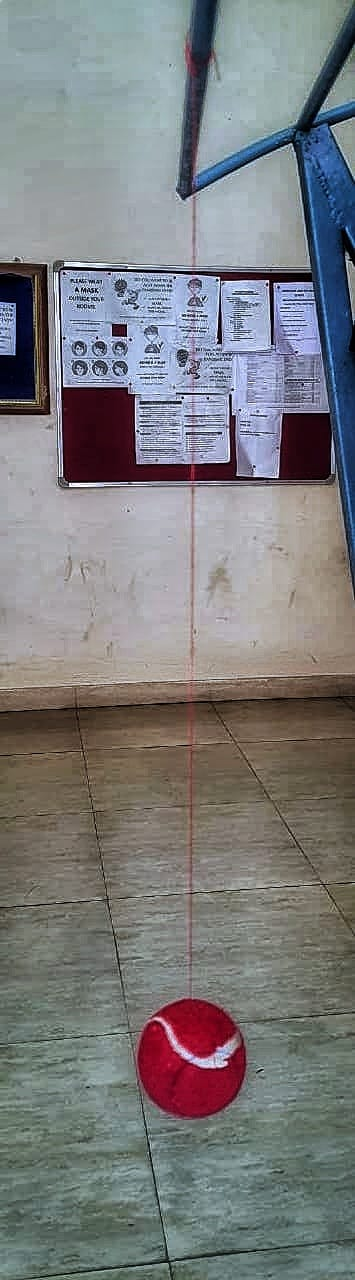
\includegraphics[scale=0.25]{Experiment}
		\caption{Image of the Setup}
	\end{figure}

	
	First a thread was hung from a rigid support (here, cloth hanger). Then, a ball was tied to the free end of the string as a bob. Then, we measure the time taken for 20 oscillations (5 to 6 readings) by taking different lengths of the string. After that we try to calculate the value of \emph{g} (acceleration due to gravity) using the formula: $$T = 2\pi \sqrt{\frac{l}{g}}$$The readings were as follows:
	
	\section{Readings/Tables}
	
	For string length 55.75 \emph{cm}:-
	
	\begin{table}[H]
		\begin{tabular}{|l|l|l|l|l|}
			\hline
			Sl. No. & Oscillations & Total Time Taken & Time per Oscillation (sec) & Average                \\ \hline
			1       & 20           & 30.26            & 1.513                      & \multirow{12}{*}{1.53} \\ \cline{1-4}
			2       & 20           & 29.50            & 1.475                      &                        \\ \cline{1-4}
			3       & 20           & 30.89            & 1.5445                     &                        \\ \cline{1-4}
			4       & 20           & 30.76            & 1.538                      &                        \\ \cline{1-4}
			5       & 20           & 30.55            & 1.5275                     &                        \\ \cline{1-4}
			6       & 20           & 30.72            & 1.536                      &                        \\ \cline{1-4}
			7       & 20           & 31.20            & 1.56                       &                        \\ \cline{1-4}
			8       & 20           & 30.9             & 1.545                      &                        \\ \cline{1-4}
			9       & 20           & 30.19            & 1.5095                     &                        \\ \cline{1-4}
			10      & 20           & 30.75            & 1.5375                     &                        \\ \cline{1-4}
			11      & 20           & 30.35            & 1.5175                     &                        \\ \cline{1-4}
			12      & 20           & 30.99            & 1.5495                     &                        \\ \hline
		\end{tabular}
	\end{table}

	For string length 71.25 \emph{cm}:-

	\begin{table}[H]
		\begin{tabular}{|l|l|l|l|l|}
			\hline
			Sl. No. & Oscillations & Total Time Taken & Time per Oscillation (sec) & Average               \\ \hline
			1       & 20           & 34.41            & 1.72                       & \multirow{7}{*}{1.71} \\ \cline{1-4}
			2       & 20           & 34.37            & 1.72                       &                       \\ \cline{1-4}
			3       & 20           & 34.40            & 1.72                       &                       \\ \cline{1-4}
			4       & 20           & 34.37            & 1.72                       &                       \\ \cline{1-4}
			5       & 20           & 34.21            & 1.71                       &                       \\ \cline{1-4}
			6       & 20           & 34.12            & 1.71                       &                       \\ \cline{1-4}
			7       & 20           & 34.17            & 1.71                       &                       \\ \hline
		\end{tabular}
	\end{table}

	\pagebreak

	For string length 96.05 \emph{cm}:-

	\begin{table}[H]
		\begin{tabular}{|l|l|l|l|l|}
			\hline
			Sl. No. & Oscillations & Total Time Taken & Time per Oscillation (sec) & Average               \\ \hline
			1       & 20           & 39.72            & 1.99                       & \multirow{6}{*}{1.99} \\ \cline{1-4}
			2       & 20           & 39.70            & 1.99                       &                       \\ \cline{1-4}
			3       & 20           & 39.71            & 1.99                       &                       \\ \cline{1-4}
			4       & 20           & 39.69            & 1.98                       &                       \\ \cline{1-4}
			5       & 20           & 39.72            & 1.99                       &                       \\ \cline{1-4}
			6       & 20           & 39.74            & 1.99                       &                       \\ \hline
		\end{tabular}
	\end{table}

	For string length 139.75 \emph{cm}:-

	\begin{table}[H]
		\begin{tabular}{|l|l|l|l|l|}
			\hline
			Sl. No. & Oscillations & Total Time Taken & Time per Oscillation (sec) & Average                \\ \hline
			1       & 20           & 47.87            & 2.39                       & \multirow{10}{*}{2.38} \\ \cline{1-4}
			2       & 20           & 47.57            & 2.38                       &                        \\ \cline{1-4}
			3       & 20           & 47.67            & 2.38                       &                        \\ \cline{1-4}
			4       & 20           & 47.49            & 2.37                       &                        \\ \cline{1-4}
			5       & 20           & 47.44            & 2.37                       &                        \\ \cline{1-4}
			6       & 20           & 47.32            & 2.37                       &                        \\ \cline{1-4}
			7       & 20           & 47.42            & 2.37                       &                        \\ \cline{1-4}
			8       & 20           & 47.52            & 2.38                       &                        \\ \cline{1-4}
			9       & 20           & 47.34            & 2.37                       &                        \\ \cline{1-4}
			10      & 20           & 47.47            & 2.37                       &                        \\ \hline
		\end{tabular}
	\end{table}

	\section{Calculations and Results}
	
	\begin{figure}[H]
		\centering
		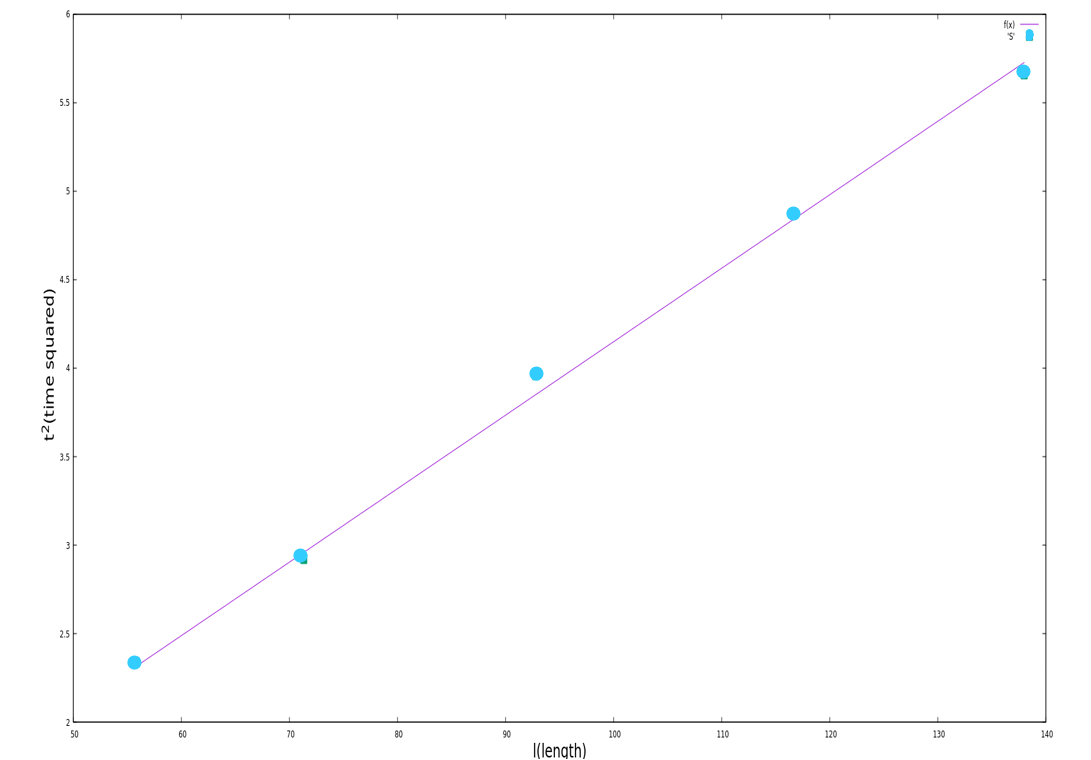
\includegraphics[scale=0.3]{photo}
		\caption{Graph of $t^{2}$ vs. $l$}
	\end{figure}

	From the formula $T = 2\pi \sqrt{\frac{l}{g}}$, we get, $$T^{2} = 4\pi^{2} \frac{l}{g}$$
	$$\Rightarrow g = 4\pi^{2} \frac{l}{T^{2}}$$
	$$Slope = \frac{T^{2}}{l} = \frac{4\pi^{2}}{g} = 0.041038\ cm^{-1} s^{2}\ (from\ graph)$$
	$$\Rightarrow \frac{4\pi^{2}}{g} = 0.041038\ cm^{-1} s^{2}$$
	$$\Rightarrow g = \frac{4\pi^{2}}{ 0.041038}\ cms^{-2} = 961.997\ cms^{-2} \approxeq 9.62\ ms^{-2}$$
	$$\boxed{g \approxeq 9.62\ ms^{-2}}$$
\end{document}